%%%%%     PACKS     %%%%%
\documentclass[12pt]{article}
\usepackage[margin=0.8in,top=0.8in,bottom=0.8in]{geometry}
\usepackage[utf8]{inputenc}
\usepackage[T1]{fontenc}
\usepackage[table, dvipsnames]{xcolor}
\usepackage{array}
\usepackage{amsmath}
\usepackage{booktabs}
\usepackage{mdframed} %For box around text
\usepackage{hyperref} %For hyperlinks in the PDF
\hypersetup{
    colorlinks=true,
    linkcolor=blue,
    filecolor=magenta,
    urlcolor=cyan,
}
\urlstyle{same}
\usepackage{amsthm}
\usepackage{amssymb}
\usepackage{amsfonts}
\usepackage{siunitx}
\usepackage{graphicx}
\usepackage{caption}
\usepackage{pgfplots}
\graphicspath{{Images/}}
\usepackage[colorinlistoftodos]{todonotes}
\usepackage{cleveref}
\usepackage[labelformat=simple]{subcaption}
\usepackage{grffile}
\usepackage{gensymb}
\usepackage{float}
\usepackage[shortlabels]{enumitem}
\usepackage{enumitem}
\setlistdepth{9}
\usepackage{biblatex} %Imports biblatex package
\addbibresource{references.bib}
\usepackage{outlines}
\usepackage{minted}
\usepackage{pdflscape}
\usepackage{everypage}
\usepackage{multirow}
\usepackage{multicol}
\usepackage{afterpage}
\usepackage[labelfont=bf, font=small]{caption}
\usepackage{upgreek}
\usepackage{tikz}
\usepackage{xcolor}
\usepackage{listings}

\usepackage{titlesec}
\titlespacing*{\section}{0pt}{6pt plus 1pt minus 1pt}{3pt}
\titlespacing*{\subsection}{0pt}{5pt plus 1pt minus 1pt}{2pt}
\titlespacing*{\subsubsection}{0pt}{4pt plus 1pt minus 1pt}{2pt}
\titlespacing*{\paragraph}{0pt}{3pt plus 1pt minus 1pt}{0.6em}

% style sheet for code
\definecolor{codegreen}{rgb}{0,0.6,0}
\definecolor{codegray}{rgb}{0.5,0.5,0.5}
\definecolor{codepurple}{rgb}{0.58,0,0.82}
\definecolor{backcolour}{rgb}{0.96,0.96,0.94}

\lstdefinestyle{mystyle}{
    backgroundcolor=\color{backcolour},   
    commentstyle=\color{codegreen},
    keywordstyle=\color{magenta},
    numberstyle=\tiny\color{codegray},
    stringstyle=\color{codepurple},
    basicstyle=\ttfamily\scriptsize,
    breakatwhitespace=false,         
    breaklines=true,                 
    captionpos=b,                    
    keepspaces=true,                 
    numbers=left,                    
    numbersep=4pt,                  
    showspaces=false,                
    showstringspaces=false,
    showtabs=false,                  
    tabsize=2,
    upquote=true,
    lineskip=-0.5pt,
    aboveskip=4pt,
    belowskip=4pt
}

\lstset{style=mystyle}

\usepackage{lastpage}
%%%%%     COMMANDS     %%%%%
%%%% Blue box for subsection text (not figures) %%%%
\newenvironment{bluebox}
  {\begin{mdframed}[backgroundcolor=blue!5,linecolor=blue!40,roundcorner=8pt]}
  {\end{mdframed}}

%%%% Simple neutral box for figures %%%%
\newenvironment{figbox}
  {\begin{mdframed}[roundcorner=8pt,shadow=true,shadowsize=4pt,shadowcolor=black!40]}
  {\end{mdframed}}

\begin{document}

\begin{titlepage}
\newcommand{\HRule}{\rule{\linewidth}{0.5mm}}

\center

\textsc{\LARGE Aarhus University}\\[1.5cm]
\textsc{\Large Department Of Computer Science}\\[0.5cm]
\textsc{\large Machine Learning}\\[0.5cm]
\textsc{\large Group 30}\\[0.5cm]
    

\HRule\\[0.4cm]
    \center 
    {\huge\bfseries  Handin 1}\\[0.4cm] % Title of your document
\HRule\\[1.5cm]

\begin{minipage}{0.4\textwidth}
        \begin{flushleft}
            \large
            \textit{Author}\\   
            Søren M. \textsc{Damsgaard}\\
            Alexander \textsc{Eriksen}\\
            Thor \textsc{Behrmann}
                 % Your name
        \end{flushleft}
    \end{minipage}
~
    \begin{minipage}{0.4\textwidth}
        \begin{flushright}
            \large
            \textit{Student number}\\
            \textbf{202309814}\\
            \textbf{202408929}\\
            \textbf{202410271}
                 % Studienummer\
            
        \end{flushright}
    \end{minipage}

\vfill\vfill\vfill % Position the date 3/4 down the remaining page
    
    {\large\today}

\vfill\vfill
    
\includegraphics[width=0.2\textwidth]{Aarhus_University_seal.png}\\[1cm] % Include a department/university logo - this will require the graphicx package
    

\vfill
\end{titlepage}
%%%%%      CHAPTERS      %%%%%
\hspace{0.02cm}
\section*{Goofy ah Machines}

\section*{PART 1: Logistic Regression}

\subsection*{Theory}

\subsubsection*{Question 1: Running Time of Mini-Batch Gradient Descent}
Let $n$ be the number of training samples, $d$ the sample dimensionality, $\text{epochs}$ the number of training epochs, and $B = \text{mini\_batch\_size}$ ($1 \le B \le n$). Multiplying an $(a \times b)$ matrix by a $(b \times c)$ matrix requires $\mathcal{O}(abc)$ time.

\textbf{Cost computation:} Given batch $X_{\text{batch}} \in \mathbb{R}^{B \times d}$, labels $y_{\text{batch}} \in \{-1, 1\}^B$, and weights $w \in \mathbb{R}^d$, computing $X_{\text{batch}} w$ takes $\mathcal{O}(B \cdot d)$ time. The element-wise product $y \odot (X_{\text{batch}} w)$ takes $\mathcal{O}(B)$. Computing $\ln(1 + e^{-y_i w^T x_i})$ via \texttt{np.logaddexp(0, -exponent)} across $B$ elements and averaging takes $\mathcal{O}(B)$. Thus, cost computation on a batch of size $B$ takes $\mathcal{O}(B \cdot d)$ time (and $\mathcal{O}(n \cdot d)$ on the full dataset of $n$ samples).

\textbf{Gradient computation:} Evaluating sigmoid values $\sigma(-y_i w^T x_i)$ and scaling by $-y_i$ takes $\mathcal{O}(B)$ time. Multiplying $X_{\text{batch}}^T$ (shape $d \times B$) by the length-$B$ vector takes $\mathcal{O}(d \cdot B)$ operations. Scaling by $1/B$ takes $\mathcal{O}(d)$. Thus, gradient computation on a batch of size $B$ takes $\mathcal{O}(B \cdot d)$ time.

\textbf{Total running time of Mini-Batch Gradient Descent (\texttt{fit}):} In each epoch, shuffling sample indices takes $\mathcal{O}(n)$ time. The dataset is partitioned into $\lceil n/B \rceil$ mini-batches; for each batch, computing the gradient takes $\mathcal{O}(B \cdot d)$ and updating weights $w \leftarrow w - \eta \nabla$ takes $\mathcal{O}(d)$. Summing across all batches yields $\frac{n}{B} \cdot \mathcal{O}(B \cdot d + d) = \mathcal{O}(n \cdot d)$. Evaluating the full in-sample cost at epoch end takes $\mathcal{O}(n \cdot d)$. Therefore, each epoch takes $\mathcal{O}(n \cdot d)$ time. Over all epochs, the total running time is:
\[
\mathcal{O}(\text{epochs} \cdot n \cdot d)
\]
Asymptotically, the running time per epoch is independent of the batch size $B$.

\subsubsection*{Question 2: Sanity Check (Pixel Permutation)}
The classifier will achieve the \textbf{exact same} performance as with the raw data. Logistic regression treats each pixel as an independent feature coordinate $x_j$ with its own weight $w_j$, without encoding 2D spatial locality (unlike CNNs). Applying any fixed permutation $\pi$ across all image pixels simply permutes feature coordinate indices ($x_{\pi(j)}$) and correspondingly permutes the learned weights ($w_{\pi(j)}$), leaving the linear inner products $w^T x = \sum_j w_j x_j$, loss function, gradient steps, and decision boundaries completely invariant.

\subsubsection*{Question 3: Linearly Separable Data}
For linearly separable data, the magnitude of the weights diverges to infinity ($\|w\| \to \infty$), while their direction converges to the maximum-margin separating hyperplane. The negative log-likelihood cost is $E_{\text{in}}(w) = \frac{1}{n}\sum_{i=1}^n \ln(1 + e^{-y_i w^T x_i})$. Since the data is linearly separable, there exists some $w^*$ such that $y_i (w^{*T} x_i) > 0$ for all $i$. Scaling $w^*$ by $c > 0$ yields:
\[
\lim_{c \to \infty} E_{\text{in}}(c w^*) = \lim_{c \to \infty} \frac{1}{n} \sum_{i=1}^n \ln(1 + e^{-c y_i w^{*T} x_i}) = 0
\]
Because the infimum of $0$ is only approached asymptotically as $c \to \infty$, gradient descent continuously takes descent steps that increase $\|w\| \to \infty$ without ever converging to finite weights.

\clearpage
\subsection*{Code}

\subsubsection*{Summary and Results}
\noindent
\begin{minipage}[c]{0.54\textwidth}
We trained the Logistic Regression classifier on the Danish CVR industry codes dataset using bag-of-words text features ($\text{epochs} = 50$, $\text{batch\_size} = 16$, $\text{lr} = 0.1$):
\begin{itemize}[noitemsep,topsep=1pt]
    \item \textbf{In-sample Accuracy:} $97.54\%$
    \item \textbf{Test Accuracy:} $95.34\%$ ($> 95\%$ target benchmark)
\end{itemize}
\textbf{Plot comments:} Cost decreases smoothly from $\sim 0.30$ to $\sim 0.08$ with stable convergence around epoch 40, verifying that $\eta = 0.1$ is well-suited.\\
\textbf{Status:} All methods pass unit tests and gradient checks.
\end{minipage}\hfill
\begin{minipage}[c]{0.43\textwidth}
    \centering
    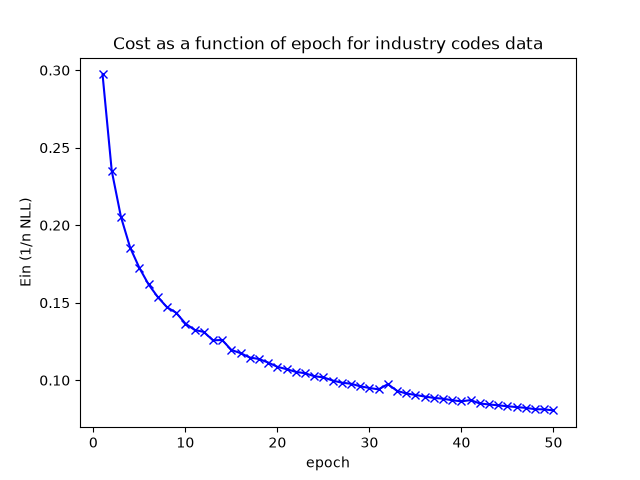
\includegraphics[width=\textwidth,height=3.2cm,keepaspectratio]{logreg_text_cost_per_epoch.png}
    \captionof{figure}{Cost ($E_{\text{in}}$) vs.\ epoch for industry codes.}
    \label{fig:logreg_cost}
\end{minipage}

\subsubsection*{Actual Code}
\begin{lstlisting}[language=Python, caption={Logistic Regression \texttt{cost\_grad} and \texttt{fit} methods.}]
def cost_grad(self, X, y, w):
    n, s = X.shape[0], y * np.dot(X, w)  # Margin: s_i = y_i * (x_i . w)
    cost = np.mean(np.logaddexp(0, -s))  # Average NLL (numerically stable)
    grad = -np.dot(X.T, y * logistic(-s)) / n  # Gradient of average NLL
    return cost, grad

def fit(self, X, y, w=None, lr=0.1, batch_size=16, epochs=10):
    if w is None: w = np.zeros(X.shape[1])
    self.history = []
    n = X.shape[0]
    for epoch in range(epochs):
        perm = np.random.permutation(n)
        for i in range(0, n, batch_size):
            b = perm[i : i + batch_size]
            _, grad = self.cost_grad(X[b], y[b], w)
            w -= lr * grad
        epoch_cost, _ = self.cost_grad(X, y, w)
        self.history.append(epoch_cost)
    self.w = w
\end{lstlisting}

\clearpage
\section*{PART 2: Softmax}

\subsection*{Theory}

\subsubsection*{Question: Running Time of Softmax Implementation}
Assume classification with $K$ classes, $n$ training samples, $d$ features, $B = \text{mini\_batch\_size}$ ($1 \le B \le n$), and $\text{epochs}$ training iterations. Multiplying an $(a \times b)$ matrix by a $(b \times c)$ matrix takes $\mathcal{O}(abc)$ time.

\textbf{Cost and Gradient in \texttt{cost\_grad}:}
For mini-batch $X \in \mathbb{R}^{B \times d}$, targets $y \in \{0, \dots, K-1\}^B$, and weights $W \in \mathbb{R}^{d \times K}$:
one-in-$K$ encoding $Y_k$ takes $\mathcal{O}(B \cdot K)$; logits $XW$ multiplies $(B \times d)$ by $(d \times K)$ taking $\mathcal{O}(B \cdot d \cdot K)$ operations; row-wise softmax probabilities $P$ (max-subtraction, exponentiation, sum, normalization) take $\mathcal{O}(B \cdot K)$; cost $-\frac{1}{B}\sum_{i,k} Y_{ik}\ln P_{ik}$ takes $\mathcal{O}(B \cdot K)$; gradient $\frac{1}{B}X^T(P - Y_k)$ multiplies $(d \times B)$ by $(B \times K)$ taking $\mathcal{O}(d \cdot B \cdot K)$ operations and $\mathcal{O}(d \cdot K)$ for scaling.
Thus, \texttt{cost\_grad} runs in $\mathcal{O}(B \cdot d \cdot K)$ time per mini-batch (and $\mathcal{O}(n \cdot d \cdot K)$ on the full dataset).

\textbf{Total running time of Mini-Batch Gradient Descent (\texttt{fit}):}
In each epoch, shuffling takes $\mathcal{O}(n)$ time. Processing all $\lceil n/B \rceil$ mini-batches takes $\sum_{j=1}^{\lceil n/B \rceil} \mathcal{O}(B \cdot d \cdot K + d \cdot K) = \mathcal{O}\left(\frac{n}{B} \cdot B \cdot d \cdot K\right) = \mathcal{O}(n \cdot d \cdot K)$. Evaluating the full in-sample cost at epoch end takes $\mathcal{O}(n \cdot d \cdot K)$.
Across all $\text{epochs}$, the total running time is:
\[
\mathcal{O}(\text{epochs} \cdot n \cdot d \cdot K)
\]

\subsection*{Code}

\subsubsection*{Summary and Results}
We evaluated our Softmax Classifier on both the Wine and MNIST digits datasets:
\begin{itemize}[noitemsep,topsep=1pt]
    \item \textbf{Wine Dataset} ($200$ epochs, $B=16$, $\eta=0.1$): In-sample Accuracy: $100.0\%$, Test Accuracy: $97.78\%$ ($> 90\%$ benchmark).
    \item \textbf{MNIST Digits} ($10$ epochs, $B=32$, $\eta=0.05$): In-sample Accuracy: $92.39\%$, Test Accuracy: $92.28\%$.
\end{itemize}

\begin{figure}[H]
    \centering
    \begin{subfigure}[b]{0.48\textwidth}
        \centering
        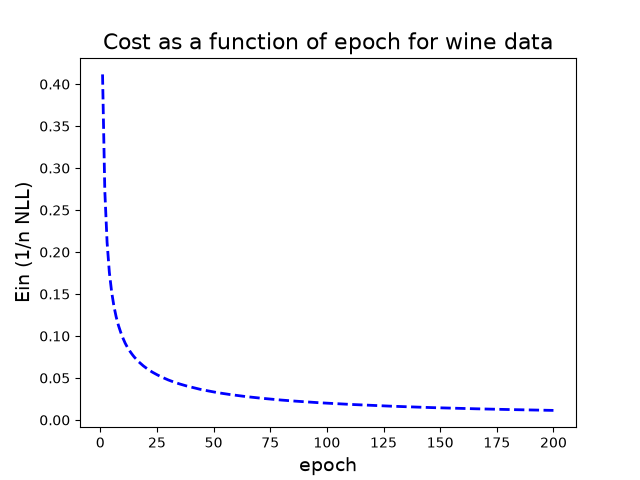
\includegraphics[height=2.8cm]{softmax_wine_cost_per_epoch.png}
        \caption{Cost per epoch on Wine data.}
        \label{fig:wine_cost}
    \end{subfigure}\hfill
    \begin{subfigure}[b]{0.48\textwidth}
        \centering
        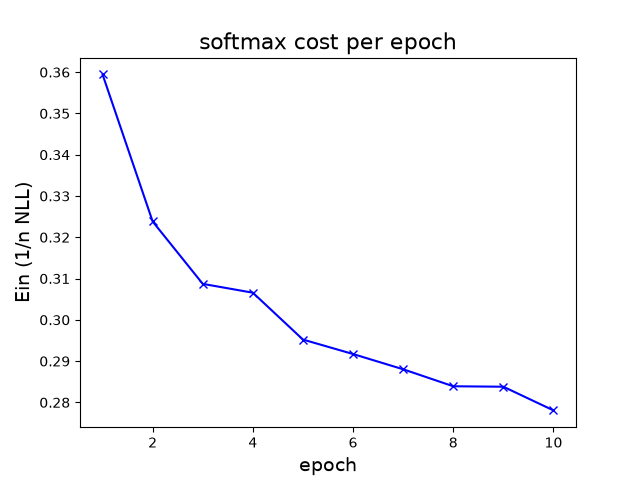
\includegraphics[height=2.8cm]{softmax_cost_per_epoch.png}
        \caption{Cost per epoch on MNIST digits.}
        \label{fig:mnist_cost}
    \end{subfigure}
    \caption{Training cost progression for Softmax regression.}
\end{figure}

\noindent\textbf{Comments on the plots:}
Both cost curves show steep initial drops followed by steady flattening without oscillations, reflecting smooth convergence. Numerical stability (log-sum-exp trick) completely prevented overflow during all runs.

\clearpage
\subsubsection*{Actual Code}
\begin{figure}[H]
    \centering
    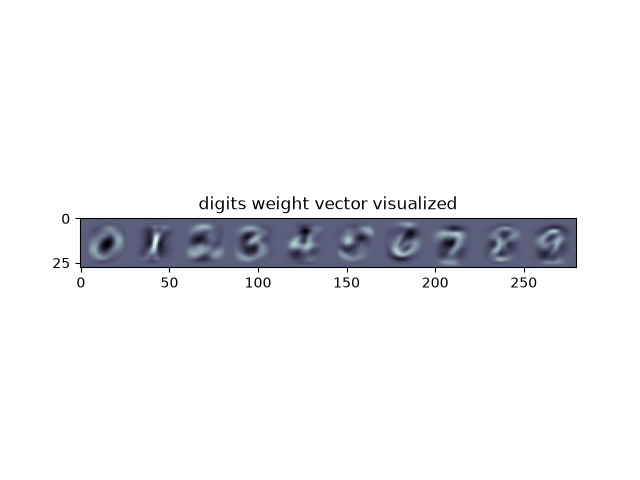
\includegraphics[width=0.75\textwidth]{softmax_weight_vector.png}
    \caption{Visualization of learned weight templates for MNIST digits $0$--$9$. Bright values correspond to positive weights matching expected stroke shapes; dark values indicate negative weights for background pixels.}
    \label{fig:weights_vis}
\end{figure}

\begin{lstlisting}[language=Python, caption={Softmax \texttt{cost\_grad} and \texttt{fit} methods.}]
def cost_grad(self, X, y, W):
    Yk = one_in_k_encoding(y, self.num_classes)
    n = X.shape[0]
    P = softmax(np.dot(X, W))
    cost = -np.sum(Yk * np.log(P)) / n  # Average NLL cost
    grad = np.dot(X.T, P - Yk) / n      # Gradient of average NLL
    return cost, grad

def fit(self, X, Y, W=None, lr=0.01, epochs=10, batch_size=16):
    if W is None: W = np.zeros((X.shape[1], self.num_classes))
    self.history = []
    n = X.shape[0]
    for epoch in range(epochs):
        perm = np.random.permutation(n)
        for i in range(0, n, batch_size):
            b = perm[i : i + batch_size]
            _, grad = self.cost_grad(X[b], Y[b], W)
            W -= lr * grad
        epoch_cost, _ = self.cost_grad(X, Y, W)
        self.history.append(epoch_cost)
    self.W = W
\end{lstlisting}

\end{document}